\documentclass[12pt]{beamer}
\usepackage{hyperref}
\usepackage[english]{babel}	
\usepackage[latin1]{inputenc}
\usepackage[T1]{fontenc}
\usepackage{lipsum}
\usepackage{bbold}
\usepackage{tcolorbox}
\tcbuselibrary{breakable}
\hypersetup{pdfpagemode=FullScreen}
\tcbuselibrary{breakable}
\definecolor{mygreen}{rgb}{.125,.5,.25}
\usecolortheme[named=mygreen]{structure}
\setbeamercolor{mycolor}{fg=white,bg=green!50}
\usetheme[secheader]{Boadilla}
\usepackage{color}
\usepackage{fancyhdr}
\usepackage{amsfonts}
\usepackage{amsmath}
\usepackage{array}
\usepackage{xcolor}
\usepackage{colortbl}
%%%%%%%%%%%%%%%%%%%%%%%%%%%%%%%%%%%%%%%%%%%%%%%%
\newcommand{\ceil}[1]{\left\lceil #1 \right\rceil}
%%%%%%%%%%%%%%%%%%%%%%%%%%%%%%%%%%%%%%%%%%%%%%%%%%%%%%%ù
%\input{mabbrev}
\usepackage{tcolorbox}
\tcbuselibrary{breakable}
%%%%%%%%%%%%%%%%%%%%%%%%%%%%%%%%%%%%%%%%%%%%
\setbeamercolor{frametitle}{bg=mygreen, fg=white}

\setbeamertemplate{blocks}[rounded,shadow=True]
%\setbeamercolor{block title example}{fg=white,bg=pink}
%\setbeamercolor{block title}{fg=white,bg=cyan}
%\setbeamercolor{block title alerted}{fg=white,bg=purple}
\author{\textbf{Candidates:} GROUP 1\\
	\textbf{Lecturer:} Prof. Wolfgang Sherer }
\title[Maths of QC]{Mathematics of Quantum Computing}
\subtitle{Group Assignment: Exercise 1}
\institute{AIMS Cameroon (African Institute for Mathematical Sciences)}
\logo{
\includegraphics[scale=0.2]{Figures/AIMSCameroonlogo}}
	\setbeamersize{text margin left=3mm, text margin right=5mm  }
\setbeamercolor{title}{bg=mygreen,fg=white}
\setbeamercovered{transparent}



%%%%%%%%%%%%%%%%%%%%tensor product%%%%%%%%%%%%%%%%%%%%%


%%%%%%%%%%%%%%%%%%%%%%%Shorcut commands%%%%%%%%%%%%%%%%%%%%%%%%%%%%%%%%%
\newcommand{\no}[1]{||#1||}
\newcommand{\ket}[1]{|#1\rangle}
\newcommand{\bra}[1]{\langle #1 |}
\newcommand{\av}[1]{\langle{#1}\rangle} %Average
\newcommand{\avp}[1]{\langle{#1}\rangle_{\psi}}
\newcommand{\kb}[2]{|#1\rangle\langle#2|} %ketbra
\newcommand{\proj}[1]{\ket{#1}\bra{#1}} % Projecteur
\newcommand{\bk}[2]{\langle#1\ket{#2}} %braket
\newcommand{\mel}[3]{\bra{#1}#2\ket{#3}} %Matrix element
\newcommand{\ep}{\hat{e}_p} 
\newcommand{\fq}{\hat{f}_q} 
\newcommand{\ddt}[1]{\frac{\mathrm{d}#1}{\mathrm{d}t}} 
\newcommand\norm[1]{\lVert#1\rVert}
\newcommand{\X}{\mathtt{X}} 
\newcommand{\HH}{\mathtt{H}} 
\newcommand{\I}{\mathbb{I}} 
\newcommand{\kup}{|\uparrow_{\vec{\hat{n}}}\rangle} 
\newcommand{\pup}{|\downarrow_{\vec{\hat{n}}}\rangle}
\newcommand{\bup}{\langle\uparrow_{\hat{n}} |} 
\newcommand{\hpsi}{\hat{\Psi}_{pq}}
\newcommand{\hphi}{\hat{\Phi}_{pq}}
\newcommand{\six}{\sigma_x}
\newcommand{\siy}{\sigma_y}
\newcommand{\siz}{\sigma_z}


\newcommand{\eqt}[1]
{\begin{equation}#1
\end{equation}}


%%%%%%%%%%%%%%%%%%Shorcut for the imbrication between environemnt equation and thet environment split%%%%%%%%%%%%%%%%%
\newcommand{\eqtt}[1]
{\begin{equation} \begin{split}#1
\end{split}\end{equation}}

\newcommand{\eqalign}[1]
{ \begin{align}#1
\end{align}}

\newcommand{\eqtta}[1]
{\begin{equation} \left\{\begin{split}#1
	\end{split}\end{equation}\right. }

\begin{document}

\begin{frame}
	\transdissolve
	\titlepage
\end{frame}
%\setbeamertemplate{frametitlecontinuation}{\insertcontinuationcount}
\begin{frame}[allowframebreaks]{Group Members}
	\begin{itemize}
	\item Peniel 
	\item Kevin
	\item Caleb
	\item Rodrigue
	\item Souleymane
	\end{itemize}
	\end{frame}
\begin{frame}[allowframebreaks]{Question 1}
	Let's determine the matrix representation of $U$.
	\begin{itemize}
	\item \eqt{U: {}^\mathrm{q}\mathbb{H}^{\otimes2}\rightarrow {}^\mathrm{q}\mathbb{H}^{\otimes2}.}
	\eqt{U\ket{00}=\ket{\Psi^+}}
	\item \textbf{Step 1} 	We apply the gate $\X$ on the second qubit and the identity to the first qubit
		\eqtt{
		(\mathbb{I}\otimes \X)\ket{00}&=\I\ket{0}\otimes \X\ket{0},\\
		&=\ket{0}\otimes\ket{1}.}
	\item \textbf{Step 2}\\
	We apply the Hadamard operator $\HH\otimes \I$ on the result of the first step to obtain :
	\eqtt{
		\HH\otimes 1\ket{01}&=\HH\ket{0}\otimes\ket{1},\\
		&=\frac{1}{\sqrt{2}}(\ket{0}+\ket{1})\otimes\ket{1}	, \text{ since } \HH\ket{0}=\frac{1}{\sqrt{2}}(\ket{0}+\ket{1}),\\
		&=\frac{1}{\sqrt{2}}(\ket{01}+\ket{11}).
	}
\item \textbf{Step 3}\\		
We apply the \textbf{CNOT-gate}. The operator $\Lambda^1(\X)$ is a 2-qubit gate such that when it is applied, the second qubit is flipped when the first qubit is the state 1, and remains the same when the first qubit is in the state 0.
\eqtt{
	\Lambda^1(\X)\frac{1}{\sqrt{2}}(\ket{01}+\ket{11})&=\frac{1}{\sqrt{2}}\left(\Lambda^1 (\X)\ket{01}+\Lambda^1(\X)\ket{11} \right)\\ 
	&=\frac{1}{\sqrt{2}}(\ket{01}+\ket{10})\\
	&=\ket{\Psi^+}.}
\begin{figure}[!h]
	\centering
	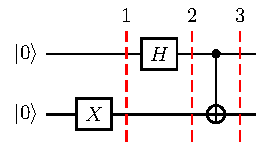
\includegraphics[scale=1.5]{Figures/circuit}
	\caption{Quantum circuit of U.}
\end{figure}
\end{itemize}
\end{frame}
\begin{frame}[allowframebreaks]{Question 2}
\begin{itemize}
\item Matrix of $U$ in the computational basis:
\eqt{U=\Lambda^1 (\X)\left( \HH\otimes\mathbb{\I}\right) \left(\I\otimes \X \right).}
We have:
\eqt{
	\I\otimes \X =
	\begin{pmatrix}
		1.\X&0.\X\\
		0.\X&1.\X
	\end{pmatrix}
	=\begin{pmatrix}
		1.\begin{pmatrix}0&1\\1&0 \end{pmatrix}&0.\begin{pmatrix}0&1\\1&0 \end{pmatrix}\\
		0.\begin{pmatrix}0&1\\1&0 \end{pmatrix}&1.\begin{pmatrix}0&1\\1&0 \end{pmatrix}
	\end{pmatrix}=
	\begin{pmatrix}
		0&1&0&0\\
		1&0&0&0\\
		0&0&0&1\\
		0&0&1&0
	\end{pmatrix}.}
Also, 
\eqtt{
	\HH\otimes\I &=\frac{1}{\sqrt{2}} \begin{pmatrix}
		1&1\\
		1&-1
	\end{pmatrix}\otimes\begin{pmatrix}
		1&0\\
		0&1
	\end{pmatrix},\\
	&=\frac{1}{\sqrt{2}} \begin{pmatrix}
		1.\I&1.\I\\
		1.\I&-1.\I
	\end{pmatrix}\\&=\frac{1}{\sqrt{2}}\begin{pmatrix}1.\begin{pmatrix}
			1&0\\
			0&1
		\end{pmatrix}&
		1.\begin{pmatrix}
			1&0\\
			0&1
		\end{pmatrix}\\1.\begin{pmatrix}
			1&0\\
			0&1
		\end{pmatrix}&
		-1.\begin{pmatrix}
			1&0\\
			0&1
	\end{pmatrix}\end{pmatrix}\\
	&=\frac{1}{\sqrt{2}} \begin{pmatrix}
		1&0&1&0\\
		0&1&0&1\\
		1&0&-1&0\\
		0&1&0&-1
\end{pmatrix}}
And,
\eqtt{
	\Lambda^1(\X)&=\ket{0}\bra{0}\otimes\I+\ket{1}\bra{1}\otimes \X,\\\\
	&=\begin{pmatrix}
		1&0\\
		0&0
	\end{pmatrix}\otimes\I+\begin{pmatrix}
		0&0\\
		0&1
	\end{pmatrix}\otimes \X,\\\\
	&=\begin{pmatrix}
		1&0&0&0\\
		0&1&0&0\\
		0&0&0&0\\
		0&0&0&0
	\end{pmatrix}+\begin{pmatrix}
		0&0&0&0\\
		0&0&0&0\\
		0&0&0&1\\
		0&0&1&0
	\end{pmatrix},}
\end{itemize}
\end{frame}
\begin{frame}[allowframebreaks]{Question 2}
	\eqt{=\begin{pmatrix}
		1&0&0&0\\
		0&1&0&0\\
		0&0&0&1\\
		0&0&1&0
	\end{pmatrix}.}\end{frame}
\begin{frame}[allowframebreaks]{Question 2}
	\begin{itemize}
\item Now given that: \eqt{U=\Lambda^1(\X)\left( \HH\otimes\I\right)\left(\I\otimes \X \right).}
Then we have that:
\eqtt{
	U&=\frac{1}{\sqrt{2}}\begin{pmatrix}
		0&1&0&0\\
		1&0&0&0\\
		0&0&0&1\\
		0&0&1&0
	\end{pmatrix}\begin{pmatrix}
		1&0&1&0\\
		0&1&0&1\\
		1&0&-1&0\\
		0&1&0&-1
	\end{pmatrix}\begin{pmatrix}
		0&1&0&0\\
		1&0&0&0\\
		0&0&0&1\\
		0&0&1&0
	\end{pmatrix},\\
	&=\frac{1}{\sqrt{2}}\begin{pmatrix}
		0&1&0&0\\
		1&0&0&0\\
		0&0&0&1\\
		0&0&1&0
	\end{pmatrix}\begin{pmatrix}
		0&1&0&1\\
		1&0&1&0\\
		0&1&0&-1\\
		1&0&-1&0
	\end{pmatrix},}
\end{itemize}
\end{frame}
%
\begin{frame}[allowframebreaks]{Question 2}
	\begin{itemize}
\item \eqt{=\frac{1}{\sqrt{2}}\begin{pmatrix}
		0&1&0&1\\
		1&0&1&0\\
		1&-1&0&1\\
		0&1&0&-1
	\end{pmatrix}.
}
Therefore the matrix $U$ in the computational basis is given by:
\eqt{U=\frac{1}{\sqrt{2}}\begin{pmatrix}
		0&1&0&1\\
		1&0&1&0\\
		1&-1&0&1\\
		0&1&0&-1
	\end{pmatrix}.}
\end{itemize}
\end{frame}
\begin{frame}{Questions 3\&4}
	\begin{itemize}
\item See Python code. 
\item See Python code 
\end{itemize}
\end{frame}
\begin{frame}[allowframebreaks]{Questions 5}
	\begin{itemize}
		\item Show that the result is indeed $\ket{\Psi^+}$.\\
		The state vector obtained obtained while programming on qiskit is
		\eqt{\begin{pmatrix}
				0\\
				\frac{1}{\sqrt{2}}\\
				\frac{1}{\sqrt{2}}\\
				0
			\end{pmatrix}.}
		$\ket{\Psi^+}$ is given by:
		\eqtt{
			\ket{\Psi^+}&=\frac{1}{\sqrt{2}}\left( \ket{01}+\ket{10}\right) \\
			&=\frac{1}{\sqrt{2}} \left(\begin{pmatrix}
				1\\
				0
			\end{pmatrix}\otimes\begin{pmatrix}
				0\\
				1
			\end{pmatrix}+\begin{pmatrix}
				0\\
				1
			\end{pmatrix}\otimes\begin{pmatrix}
				1\\
				0
			\end{pmatrix}\right)}
		\eqtt{
			&=\frac{1}{\sqrt{2}}\begin{pmatrix}
				1.\begin{pmatrix}
					0\\
					1
				\end{pmatrix}\\
				0.\begin{pmatrix}
					0\\
					1\end{pmatrix}\end{pmatrix}+\frac{1}{\sqrt{2}}\begin{pmatrix}
				0.\begin{pmatrix}
					1\\
					0
				\end{pmatrix}\\
				1.\begin{pmatrix}
					1\\
					0
			\end{pmatrix} \end{pmatrix}\\
			&=\frac{1}{\sqrt{2}}\left(\begin{pmatrix}
				0\\
				1\\
				0\\
				0
			\end{pmatrix}+\begin{pmatrix}
				0\\
				0\\
				1\\
				0
			\end{pmatrix}\right)\\
			&=\begin{pmatrix}
				0\\
				\frac{1}{\sqrt{2}}\\
				\frac{1}{\sqrt{2}}\\
				0
			\end{pmatrix}=\ket{\Psi^+}.}
		Hence, the result obtained is indeed $\ket{\Psi^+}.$
	\end{itemize}

\end{frame}
\begin{frame}
	\centering
	\Huge{Thank you for your kind attention}
	\end{frame}
\end{document}